%% Randomised range finder on a synthetic 512x512 picture (generated by figs_c5ch02.py).
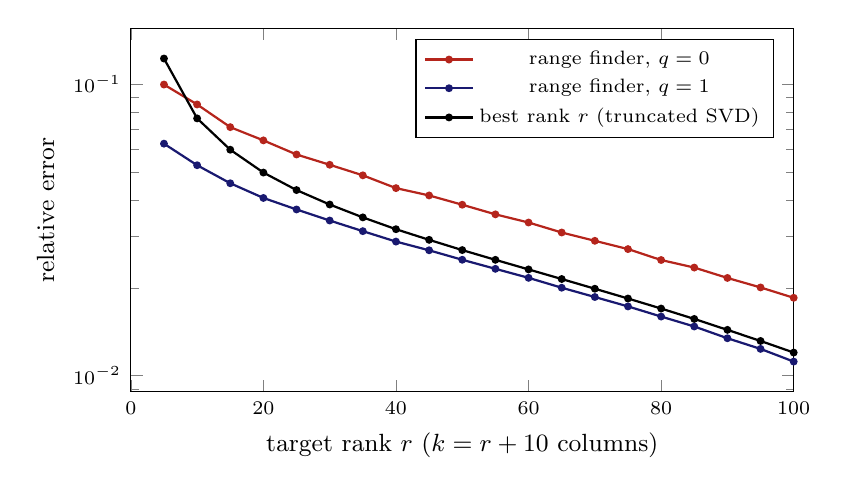
\begin{tikzpicture}
\begin{axis}[width=10cm,height=6.2cm,ymode=log,xmin=0,xmax=100,xlabel={target rank $r$ ($k=r+10$ columns)},ylabel={relative error},
  tick label style={font=\scriptsize},label style={font=\small},legend style={font=\scriptsize,at={(0.97,0.97)},anchor=north east}]
\addplot[BrickRed,thick,mark=*,mark size=1pt] coordinates {(5,9.9676e-02) (10,8.5169e-02) (15,7.1197e-02) (20,6.4113e-02) (25,5.7350e-02) (30,5.2879e-02) (35,4.8646e-02) (40,4.3971e-02) (45,4.1501e-02) (50,3.8570e-02) (55,3.5742e-02) (60,3.3510e-02) (65,3.0967e-02) (70,2.8998e-02) (75,2.7163e-02) (80,2.4915e-02) (85,2.3474e-02) (90,2.1625e-02) (95,2.0061e-02) (100,1.8486e-02)};
\addlegendentry{range finder, $q=0$}
\addplot[MidnightBlue,thick,mark=*,mark size=1pt] coordinates {(5,6.2483e-02) (10,5.2689e-02) (15,4.5693e-02) (20,4.0684e-02) (25,3.7151e-02) (30,3.4040e-02) (35,3.1298e-02) (40,2.8822e-02) (45,2.6906e-02) (50,2.4966e-02) (55,2.3241e-02) (60,2.1644e-02) (65,2.0018e-02) (70,1.8601e-02) (75,1.7270e-02) (80,1.5940e-02) (85,1.4737e-02) (90,1.3429e-02) (95,1.2344e-02) (100,1.1167e-02)};
\addlegendentry{range finder, $q=1$}
\addplot[black,thick,mark=*,mark size=1pt] coordinates {(5,1.2241e-01) (10,7.6296e-02) (15,5.9564e-02) (20,4.9726e-02) (25,4.3299e-02) (30,3.8634e-02) (35,3.4897e-02) (40,3.1783e-02) (45,2.9222e-02) (50,2.6950e-02) (55,2.4952e-02) (60,2.3131e-02) (65,2.1442e-02) (70,1.9862e-02) (75,1.8382e-02) (80,1.6981e-02) (85,1.5643e-02) (90,1.4348e-02) (95,1.3144e-02) (100,1.1992e-02)};
\addlegendentry{best rank $r$ (truncated SVD)}
\end{axis}
\end{tikzpicture}
